\section{Reweight and uncertainty of $\tau\to \rm h$ decay}

In both shape and counting analysis, signal MC events with $W\to\ell,
W\to\tau\to hadrons$ in $l\tau$ channel is essential to the sensity of
$Br(W\to\tau)$ measurement.  However, because various hadronic decay
mode of $\tau$ have different efficiency in $\tau$ reconstruction, the
selection efficiency of simulated events with $W\to l, W\to\tau\to
hadrons$ can heavily depends on the assumption of $Br(\tau\to hadrons)$
values in the MC generator.  Potential bias in the $Br(\tau\to hadrons)$
value in MC generator can affect the efficiency matrix in both shape and
counting analysis, thus propagetes to the final measurement.  This study
is to correct $Br(\tau\to hadrons)$ value assumed in MC generator with
the latest PDG values, by the reweighting signal MC events with deferent
decay mode of $\tau\to hadrons$.

In \ttbar MC sample, hard process is generated by \POWHEG while \tau
decay is handled by \PYTHIA8.  The values of $Br(\tau\to hadrons)$
assumed in \PYTHIA8 and presented in PDG are shown in
Table~\ref{tab:tauhReweighting}. The difference between values in
\PYTHIA8 and PDG is about $0.5\%$.


In tt MC sample, we save the gen-level daughtor mesons from upto two
$\tau_h$'s in hard process.  The daughtor mesons from $\tau_h$ in events
with $W\to l, W\to\tau\to hadrons$ selected in $l\tau$ channel is shown
in Fig~\ref{fig:appendix:reweightTauhBr:tauhBr}


\begin{table}[]
  \centering
  \begin{tabular}{l|c|c|c}
  \hline
                              & PDG        & PYTHIA8   & PDG / PYTHIA8 \\
  \hline
  $Br(\tau\to \pi^\pm)$       & 0.1082(5)  & 0.1076825 & 1.00481       \\
  $Br(\tau\to \pi^\pm+ \pi^0)$& 0.2549(9)  & 0.2537447 & 1.00455       \\
  $Br(\tau\to \pi^\pm+2\pi^0)$& 0.0926(10) & 0.0924697 & 1.00141       \\
  $Br(\tau\to3\pi^\pm)$       & 0.0931(5)  & 0.0925691 & 1.00574       \\
  $Br(\tau\to3\pi^\pm+ \pi^0)$& 0.0462(5)  & 0.0459365 & 1.00574       \\
  \hline
  \end{tabular}
  \caption{ The values of $Br(\tau\to hadrons)$ in PYTHIA8 and in PDG.
  \label{tab:tauhReweighting}}
\end{table}


\begin{figure}
    \centering
    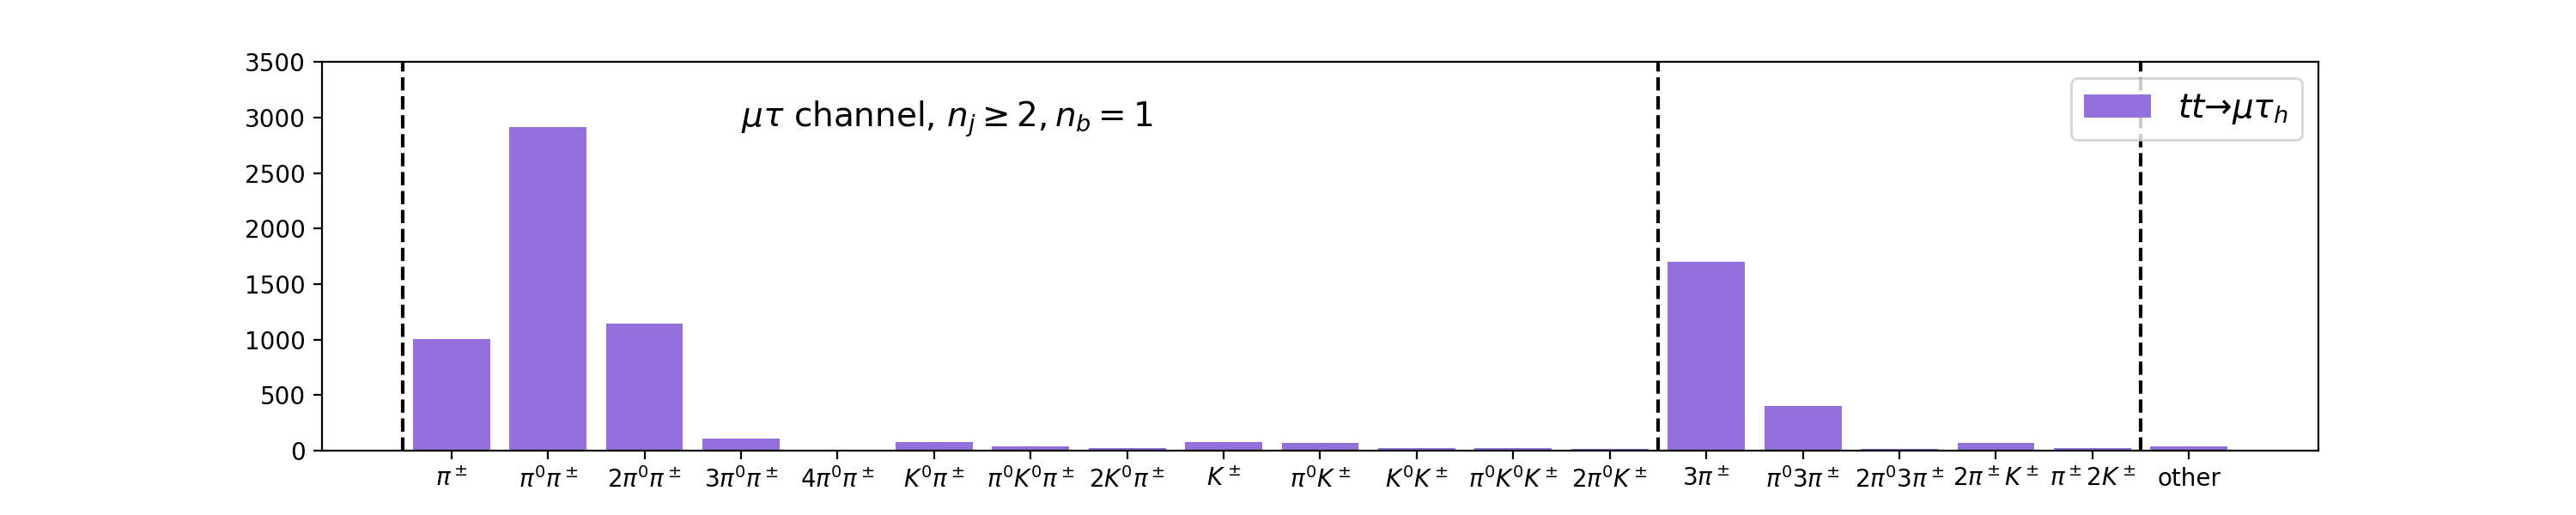
\includegraphics[width=0.99\textwidth]{chapters/Appendix/sectionTauBr/figures/tauhDecay_mutau.png}
    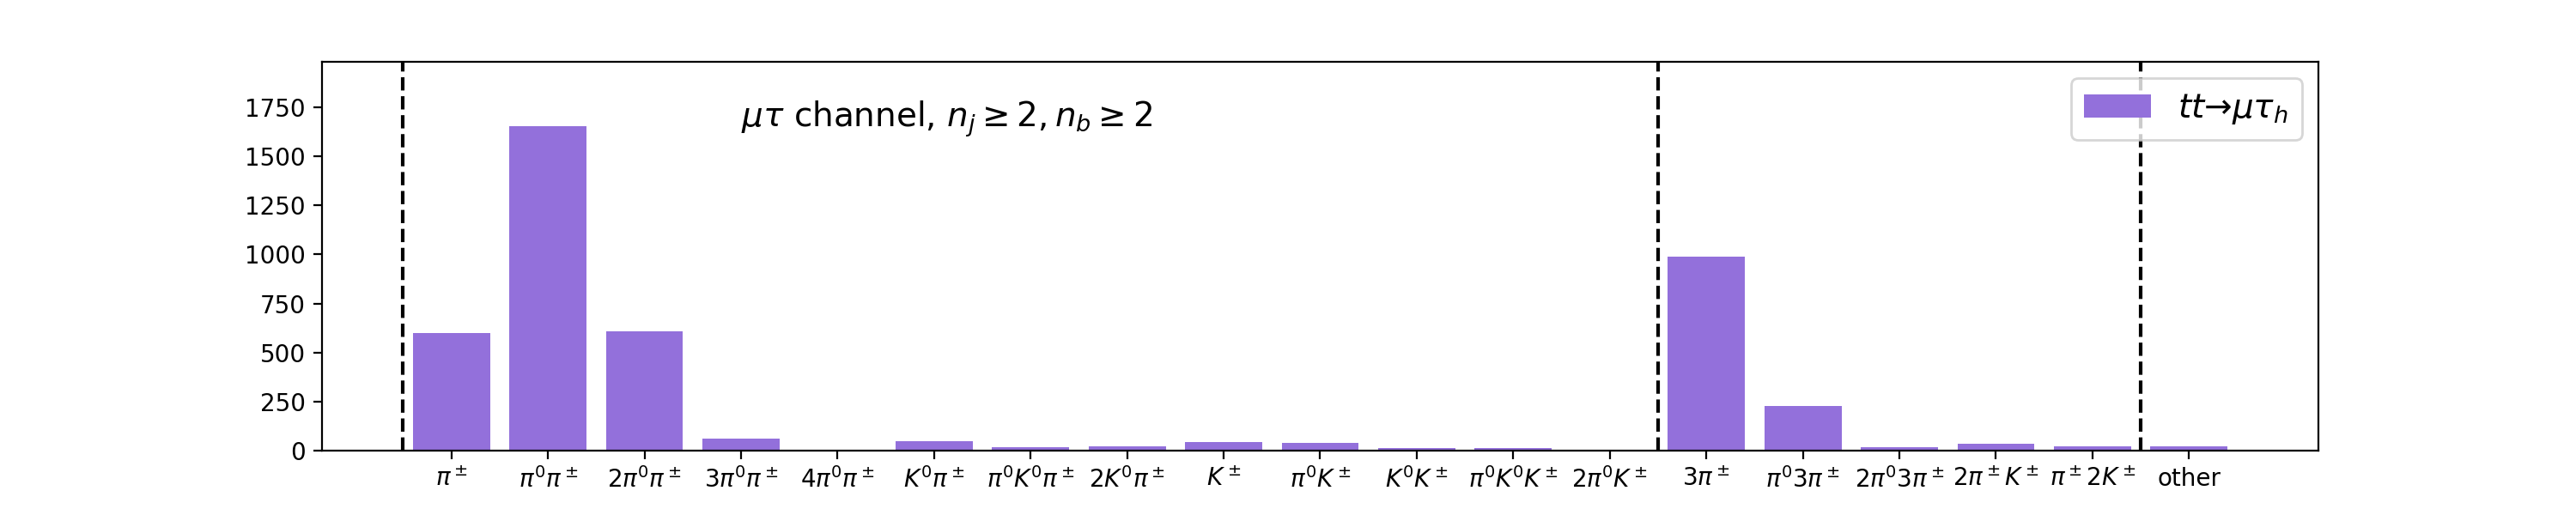
\includegraphics[width=0.99\textwidth]{chapters/Appendix/sectionTauBr/figures/tauhDecay_mutau2.png}
    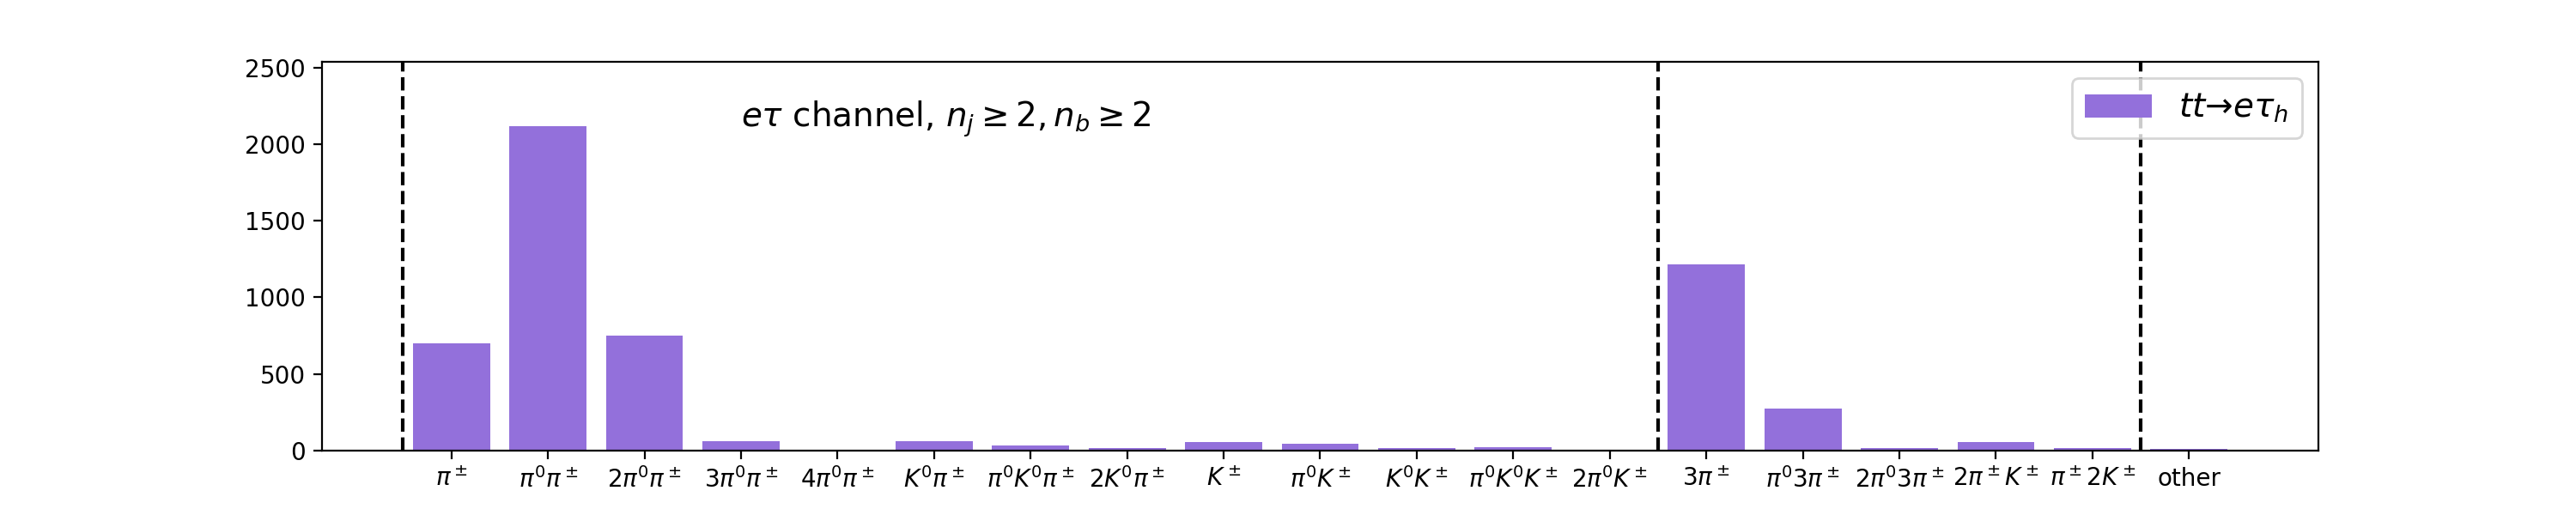
\includegraphics[width=0.99\textwidth]{chapters/Appendix/sectionTauBr/figures/tauhDecay_etau.png}
    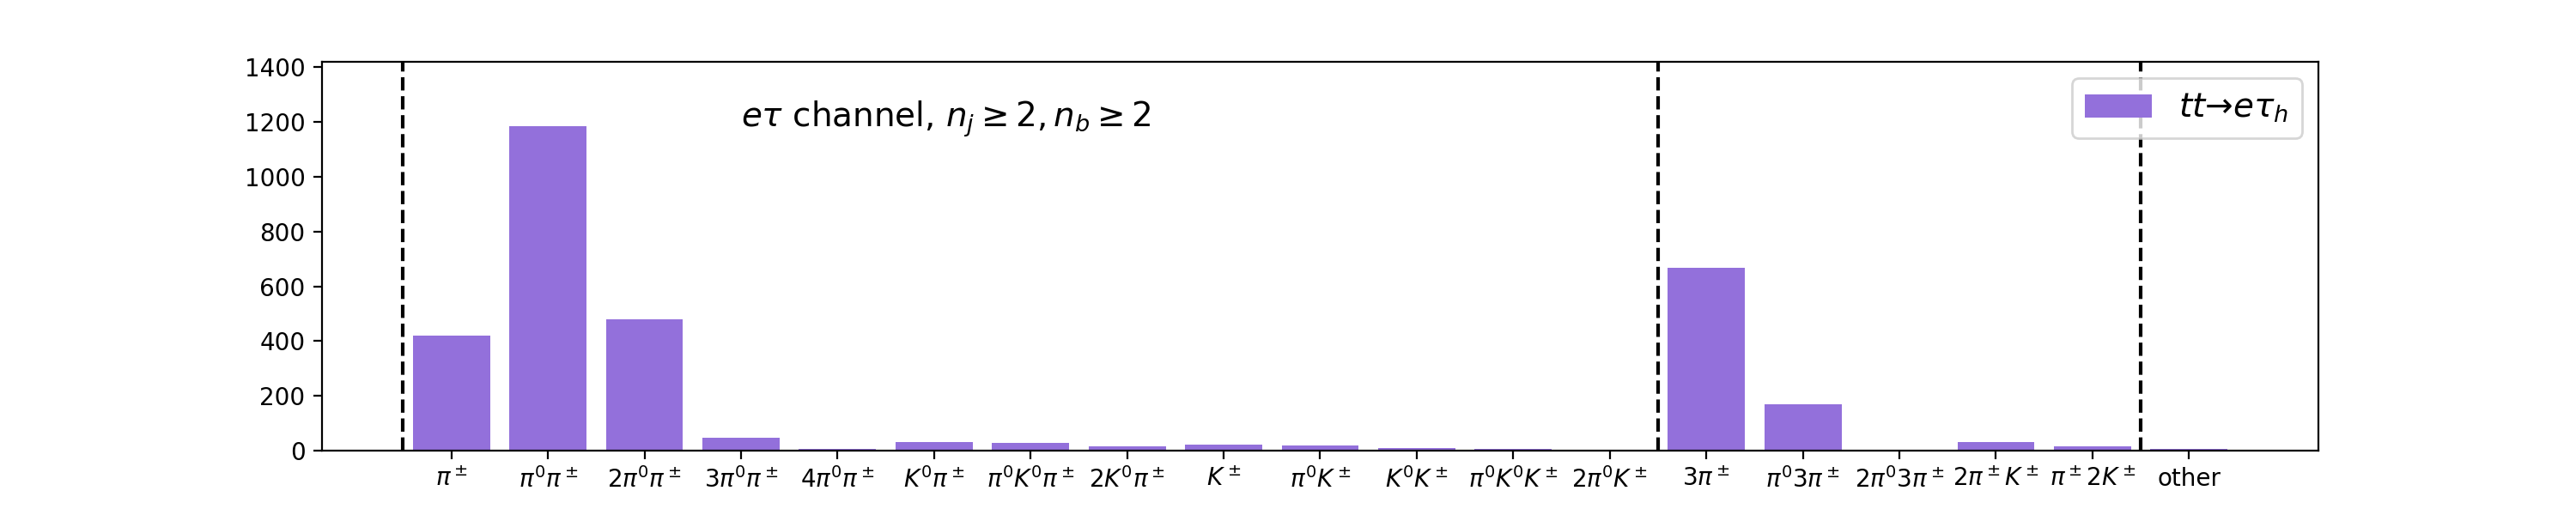
\includegraphics[width=0.99\textwidth]{chapters/Appendix/sectionTauBr/figures/tauhDecay_etau2.png}


    \caption{tauh Br}
    \label{fig:appendix:reweightTauhBr:tauhBr}
\end{figure}


The leading contributions to $l\tau$ channel are from $\tau\to
\pi^\pm+\pi^0 $, $\tau\to 3\pi^\pm$, $\tau\to \pi^\pm+2\pi^0$, $\tau\to
\pi^\pm$, $\tau\to 3\pi^\pm + \pi^0$. MC events with those five tau
decay modes are reweighted by 

\begin{equation}
  w = \frac{^{PDG} Br(\tau\ to  hadrons) }{^{PYTHIA8} Br(\tau\ to  hadrons)}
\end{equation} 

with a weight uncertainty equals to the different between PDG value and
\PYTHIA8 value

\begin{equation}
  uncertainty(w) = |^{PDG} Br(\tau\ to  hadrons) - ^{PYTHIA8} Br(\tau\ to  hadrons) |
\end{equation} 

Propagating the uncertainty of $Br(\tau\ to  hadrons)$ to the $Br(W)$
measurement, we obtain the systematic uncertainty due to $Br(\tau\ to
hadrons)$. As is shown in table \ref{tab:syst_tauhReweighting},
uncertainty of $Br(\tau\ to  hadrons)$ leads to about $0.003 - 0.146 \%$
uncertainty to $Br(W)$.

\begin{table}[p]
  \centering
  \scriptsize
  \begin{tabular}{|l|ccc|ccc|ccc|ccc|ccc|}
  \hline
  Error Source & \multicolumn{3}{c|}{$\mu$-1b} & \multicolumn{3}{c|}{$\mu$-2b} & \multicolumn{3}{c|}{$e$-1b} & \multicolumn{3}{c|}{$e$-2b} \\
  \hline
                & $B_e$ & $B_\mu$ & $B_\tau$ & $B_e$ & $B_\mu$ & $B_\tau$ & $B_e$ & $B_\mu$ & $B_\tau$ & $B_e$ & $B_\mu$ & $B_\tau$ \\
  \hline
  0.5$\%$ err of $Br_{\tau\to\pi^\pm}$       & 0.009 & 0.013 & 0.055 & 0.009 & 0.012 & 0.051 & 0.009 & 0.012 & 0.052 & 0.010 & 0.012 & 0.057 \\ 
  0.5$\%$ err of $Br_{\tau\to\pi^\pm\pi^0}$  & 0.025 & 0.033 & 0.141 & 0.026 & 0.033 & 0.147 & 0.024 & 0.032 & 0.146 & 0.025 & 0.032 & 0.146 \\ 
  0.2$\%$ err of $Br_{\tau\to\pi^\pm2\pi^0}$ & 0.003 & 0.004 & 0.017 & 0.003 & 0.004 & 0.015 & 0.003 & 0.004 & 0.017 & 0.003 & 0.004 & 0.019 \\ 
  0.6$\%$ err of $Br_{\tau\to3\pi^\pm}$      & 0.017 & 0.022 & 0.101 & 0.019 & 0.023 & 0.111 & 0.017 & 0.023 & 0.107 & 0.017 & 0.022 & 0.107 \\ 
  0.6$\%$ err of $Br_{\tau\to3\pi^\pm\pi^0}$ & 0.005 & 0.006 & 0.024 & 0.005 & 0.006 & 0.022 & 0.004 & 0.006 & 0.022 & 0.005 & 0.006 & 0.025 \\ 
  \hline
  \end{tabular}
  \caption{ systematic uncertainty ($\%$) due to $Br(\tau\ to  hadrons)$. Take the difference 
            between $Br(\tau\ to  hadrons)$ value in PDG and Pythia8 as systematic uncertainty.
            }
  \label{tab:syst_tauhReweighting}
\end{table}
\FloatBarrier